%==============================================================================
\section{Neutrino Oscillations}
\label{sec:osc}
%==============================================================================

The Standard Model of Particle Physics, as described in the previous section,
has been one of the most successful theories in the history of physics. It is,
however, not fundamental in the sense that it can explain all physical
phenomena alone. Its shortcomings are e.\,g.\ the missing inclusion of the
fourth fundamental force, gravity, and a lack of explanation for the fundamental
asymmetry between bosons and fermions.
There are theoretical extensions to the Standard Model addressing these
questions, such as ``Grand Unified Theories'', supersymmetry, and many others 
\cite{Nagashima}, but all of them lack experimental evidence so far.

Yet there is one effect of so-called ``Physics beyond the Standard Model'' that
has been well established experimentally during the past years: neutrino
oscillations. As already mentioned in Sec.~\ref{sec:NusInSM}, this term refers
to neutrinos changing their flavour when travelling over macroscopic distances,
which can be explained by finite neutrino masses, while in the Standard Model
they have zero mass.

The theory behind this process will be described in the following. In-depth
treatments of this topic can be found in many textbooks, e.\,g.\
\cite{GiuntiKim, Zuber, Nagashima, XingZhou}. In terms of notation, we will
follow \cite{GiuntiKim} here.

\subsection{Vacuum Oscillations}
\label{sec:VacOsc}

There are two bases of eigenstates to which a neutrino can be decomposed: the
flavour and the mass base. The flavour eigenstates are \ket{\nue}, \ket{\numu},
and \ket{\nutau}, which will be summarised as \ket{\nu_\alpha}. These are the
eigenstates of the weak interaction, hence neutrinos are always produced as a
pure flavour eigenstate and have to be projected back onto these eigenstates
whenever they interact.

On the other hand there are the three mass eigenstates \ket{\nu_1}, \ket{\nu_2},
and \ket{\nu_3}, summarised as \ket{\nu_k}, corresponding to the three neutrino
masses $m_k$. The absolute values of these masses are yet unknown, but since
neutrino oscillations have been observed, at least two of them have to be
different from zero. The mass eigenstates have to be considered when describing
the propagation of a neutrino in vacuum since they are the eigenstates of the
corresponding Hamiltonian
\begin{equation}
%  \hat{H} = -\frac{\hbar^2}{2m}\nabla^2
 \hat{H}\,\ket{\nu_k} = E_k\,\ket{\nu_k} \quad.
 \label{eqn:vac_hamiltonian}
\end{equation}
% only depends on its mass.

\subsubsection{General Case}

Changes between the two bases are carried out via the so-called PMNS
matrix\footnote{After Bruno Pontecorvo, Ziro Maki, Masami Nakagawa, and Shoichi
Sakata.} $\mathcal{U}_\mathrm{PMNS}$ that can be parametrised using three Euler
angles \thet{ij}, also called mixing angles, and one complex phase angle
$\delta$ that is related to possible CP violation:
\begin{equation}
 \mathcal{U}_\mathrm{PMNS} =
 \begin{pmatrix}
  U_{e1} & U_{e2} & U_{e3} \\
  U_{\mu 1} & U_{\mu 2} & U_{\mu 3} \\
  U_{\tau 1} & U_{\tau 2} & U_{\tau 3}
 \end{pmatrix}
 =
 \begin{pmatrix}
  1 & 0 & 0 \\
  0 & c_{23} & s_{23} \\
  0 & -s_{23} & c_{23}
 \end{pmatrix}
 \begin{pmatrix}
  c_{13} & 0 & s_{13}e^{-i\delta} \\
  0 & 1 & 0 \\
  -s_{13}e^{i\delta} & 0 & c_{13}
 \end{pmatrix}
 \begin{pmatrix}
  c_{12} & s_{12} & 0 \\
  -s_{12} & c_{12} & 0 \\
  0 & 0 & 1
 \end{pmatrix}
\label{eqn:PMNS}
\end{equation}
Here, $s_{ij}$ and $c_{ij}$ are shorthands for $\sin\thet{ij}$ and
$\cos\thet{ij}$, respectively. Transformations between flavour and mass base
are then given by
\begin{eqnarray}
 \ket{\nu_\alpha} = \sum_k U^*_{\alpha k}\, \ket{\nu_k}\quad, \\
 \ket{\nu_k} = \sum_\alpha U_{\alpha k}\, \ket{\nu_\alpha}\quad.
\end{eqnarray}

To ensure lepton number conservation, unitarity of $\mathcal{U}_\mathrm{PMNS}$
has to be required. Any deviation from this can be interpreted as a hint for
additional neutrino flavours that do not participate in the weak
interaction\footnote{Measurements of the $Z^0$ decay width have shown that only
three weakly interacting neutrino flavours exist \cite{Zwidth}---at least at
masses up to half the $Z^0$ mass, $m_\nu < m_{Z^0}/2 = 45.6$\,GeV.}. Such
signals have been reported (e.\,g.\ \cite{MiniBooNE}), but the overall
picture remains inconclusive \cite{PDG}.

% TODO: Make Hamiltonian matrix formalism more clear

If now a pure flavour eigenstate \ket{\nu_\alpha} is produced at an energy $E$,
the probability to detect it as \ket{\nu_\beta} after propagating over a
distance $L$ has to be calculated according to
\begin{equation}
 P_{\alpha\to\beta} = \left|\Braket{\nu_\beta
                            \left|\,\mathcal{U}^\dagger\,\left|\,\hat{H}
                             \,\right|\,\mathcal{U}\,\right|
                             \nu_\alpha}\right|^2 \quad.
 \label{eqn:osc_prob_hamiltonian}
\end{equation}
In the mass base, the propagation of the neutrinos can be described as plain
waves,
\begin{equation}
 \Ket{\nu_k(t)} = \exp\left(-i(E_k t - \vec{p}_k\cdot \vec{x})\right)\,
  \Ket{\nu_k(0)} \quad,
\end{equation}
and assuming relativistic neutrinos ($m_k \ll E_k \Rightarrow v \approx c$) one
can approximate in natural units\footnote{$\hbar = c = 1$}
\begin{eqnarray}
 E_k =       \sqrt{ \vec{p}_k^2 - m_k^2 }
     \approx p_k + \frac{m_k^2}{2p_k} \quad, \\
 E_k t - \vec{p}_k\cdot \vec{x} = \left(p_k + \frac{m_k^2}{2p_k}\right) L
                                  - p_k L \approx \frac{m_k^2}{2E} L
\end{eqnarray}
With this, (\ref{eqn:osc_prob_hamiltonian}) reduces to
\begin{equation}
 P_{\alpha\to\beta} = \sum_{k,j} U^*_{\alpha k} U_{\beta k} U_{\alpha j}
                        U^*_{\beta j}
                        \exp\left( -i\frac{\dm{kj}L}{2E} \right)
 \label{eqn:osc_prob_reduced}
\end{equation}
with the squared mass differences
\begin{equation}
 \dm{kj} \equiv m^2_k - m^2_j \quad.
\end{equation}
Here we note that obviously in the mass base the Hamiltonian can be replaced by
an effective one containing the squared masses:
\begin{equation}
 \hat{H}^\mathrm{eff}
 = \frac{1}{2E}\,\mathrm{diag}\left(m_1^2,\,m_2^2,\,m_3^2\right)
 = \frac{m_1^2}{2E}\mathlarger{\mathlarger{\mathbbm{1}}} +
   \frac{1}{2E}\,\mathrm{diag}\left(0,\,\dm{21},\,\dm{31}\right)
 \label{eqn:vac_eff_hamiltonian}
\end{equation}
We can even ignore the first summand on the r.\,h.\,s.\ of the above equation
since it will only introduce an unobservable global phase shift. This
simplification will prove handy when discussing oscillations in matter in
Sec.~\ref{sec:matter_osc}.

Using the unitarity of $\mathcal{U}_\mathrm{PMNS}$, (\ref{eqn:osc_prob_reduced})
can now be rewritten as
\begin{eqnarray}
 P_{\alpha\to\beta} = \delta_{\alpha\beta}
                      &-& 2\sum_{k>j} \Re\left[ U^*_{\alpha k} U_{\beta k}
                                              U_{\alpha j} U^*_{\beta j} \right]
                                    \left[1-\cos \frac{\dm{kj}L}{2E} \right]
                                    \nonumber \\
                      &+& 2\sum_{k>j} \Im\left[ U^*_{\alpha k} U_{\beta k}
                                              U_{\alpha j} U^*_{\beta j} \right]
                                    \sin \frac{\dm{kj}L}{2E} \quad.
\end{eqnarray}

Obviously, this oscillation probability collapses to $P_{\alpha\to\beta} =
\delta_{\alpha\beta}$ if all $m_i$ are equal. Hence the observation of actual
flavour conversion means that the $m_i$ are different from each other and in
particular different from zero (at least two of them), contradicting the
standard model prediction of vanishing neutrino masses. Additionally, the
second oscillatory term only contributes if there is CP violation in
the neutrino sector---otherwise the mixing matrix (\ref{eqn:PMNS}) is real.

For antineutrinos, the oscillation probability is derived analogously, only
with $\mathcal{U}_\mathrm{PMNS}$ being replaced by its complex conjugate. Hence
differing vacuum oscillation probabilities for neutrinos and antineutrinos are
a proof of CP violation.

\subsubsection{Two Flavour Case}

In many cases\footnote{In particular, if the survival probability of a certain
flavour is measured.} it is sufficient to consider only two neutrino flavours in
the oscillation. Then there is only one mass splitting
\begin{equation}
 \dm{} \equiv \dm{21} \equiv m^2_2 - m^2_1
\end{equation}
and the mixing matrix $\mathcal{U}$ can be parametrised by one effective mixing
angle
\begin{equation}
 \mathcal{U} =
 \begin{pmatrix}
 \cos\vartheta & \sin\vartheta \\
 - \sin\vartheta & \cos\vartheta
 \end{pmatrix} \quad.
\end{equation}
The expression for the transition probability simplifies to
\begin{equation}
 P_{\alpha\to\beta} = \sin^2 2\vartheta \sin^2\left( \frac{\dm{}L}{4E} \right)
                    = \sin^2 2\vartheta\sin^2\left(\pi\frac{L}{L^\mathrm{osc}}
                       \right) \qquad (\alpha \neq \beta) \quad,
 \label{eqn:twoflavour_prob}
\end{equation}
introducing the oscillation length
\begin{equation}
 L^\mathrm{osc} \equiv \frac{4\pi\,E}{\dm{}}
  \approx 2.47 \frac{E\,[\si{\GeV}]}{\dm{}\,[\si{\eVsq}]} \si{\km}  \quad.
\end{equation}

From (\ref{eqn:twoflavour_prob}), the two different groups of parameters in
neutrino oscillation phenomenology and how they influence the oscillation
probabilities, become obvious:
The mixing angles define the amplitude of the oscillation, with $\vartheta
\approx \ang{45}$ giving rise to so-called ``maximum mixing'' where a full
transition from one flavour to another is possible. The mass splittings
determine the frequency at a given neutrino energy, expressed through the
oscillation length at which the first full oscillation cycle is completed.

So from an experimental point of view, placing a detector at a distance $L =
L^\mathrm{osc}/2$ from the neutrino source is preferential, since here the
oscillation effects are strongest. If $L \ll L^\mathrm{osc}$, the flavour
transition has not yet happened while at $L \gg L^\mathrm{osc}$ only the
average transition probability
\begin{equation}
 \left\langle P_{\alpha\to\beta} \right\rangle
  = \frac{1}{2}\sin^2 2\vartheta
\end{equation}
can be measured and no information on \dm{} can be obtained\footnote{Here it
is assumed that in a real experiment one will always have a continuous
neutrino energy spectrum and hence a distribution of oscillation lengths.
Hence the fast oscillations will smear out on a distance $L \gg
L^\mathrm{osc}$.}.

\subsection{Absolute Neutrino Masses and Mass Hierarchy}
\label{sec:NMH}

Since the existence of neutrino oscillations has unambiguously shown that 
neutrinos have non-zero masses, the question is what the absolute values of 
these masses are. Although this question seems to be very simple, it turns out 
to be experimentally very challenging.

To establish absolute neutrino masses one has to consider effects such 
as distortions at the upper end of the energy spectrum of nuclear $\beta$ 
decays (as described in Sec.~\ref{sec:BetaDecay}). Here the decay of tritium is 
promising due to its small decay energy. In fact, currently the most stringent 
upper limits for the mass of the electron (anti-) neutrino
\footnote{Defined as $m_{\nue}^2 = \sum_i 
|U^2_{ei}|\, m_i^2$ \cite{NuMassReview}.} set by the Mainz and Troitsk 
experiments \cite{MainzNuMass, TroitskNuMass} stem from this very decay. Their 
limit of 
\begin{equation}
 m_{\nuebar} \lesssim \SI{2.1}{\eV}
\end{equation}
is expected to be improved by one order of magnitude in the KATRIN experiment 
that targets the tritium decay spectrum as well \cite{KATRIN}.

However these experiments can only directly measure the superposition of mass
eigenstates that corresponds to the \nue or \nuebar flavour eigenstate. A direct
measurement of the \numu or \nutau mass (or their antiparticles) is by far more
difficult since they cannot be created in a controllable source like a nuclear
decay. The only not completely unrealistic options here would be time-of-flight
measurements with an extremely long baseline\footnote{E.\,g.\ astrophysical
neutrinos that can be associated with a transient event such as a supernova or a
gamma-ray burst.}. 

So the most promising overall approach is to fix the neutrino mass scale at one 
point by measuring the \nue mass directly and then derive the other mass 
eigenstates via the mass differences that are accessible in neutrino 
oscillations. On the other hand, apart from CP violating effects, which have not 
yet been observed, all oscillatory terms above are proportional to either $\cos$ 
or $\sin^2$ and hence insensitive to the sign of their argument.
Thus, in vacuum oscillations, only information on the distances of the mass 
eigenstates can be collected, but not on their relative ordering or 
\emph{hierarchy}. 

% In other words, studying oscillations one can measure the difference between 
% e.\,g.\ the (squared) mass eigenstates $m_1$ and $m_2$, but not their actual 
% values and not even whether $m_2$ is larger or smaller than $m_1$---the ordering 
% or \emph{hierarchy} of the masses.

This could be resolved, however, if one would measure all three mass
splittings separately and then use that obviously
% (\ref{eqn:mass_diff_link}) 
\begin{equation}
 \dm{31} = \dm{32} + \dm{21} \quad.
 \label{eqn:mass_diff_link}
\end{equation}
to derive the ordering. Unfortunately, it turns out \cite{Fogli, 
GonzalezGarcia} that
\begin{equation}
 \dm{32} \simeq \dm{31} \gg \dm{21} \quad,
\end{equation}
such that with current experiments' precision it is impossible to disentangle
\dm{32} and \dm{31}. So what can be done to learn about the ordering of the 
neutrino mass eigenstates?

There is a possibility to access the neutrino mass hierarchy in oscillation
experiments, if the neutrinos in question pass through a sufficient amount of
matter along their path. In this case, additional resonances appear that depend
on the sign of the mass splittings. These so-called matter effects will be
discussed in the following section.


% Although the existence of neutrino masses is essential for neutrino 
% oscillations, the relevant parameters are not the three mass eigenstates 
% themselves, but their squared differences \dm{kj}. So they are not three, but 
% only two independent parameters since obviously
% 
% 
% 
% Thus oscillations are needed to establish the relative
% positions of the mass eigenstates. But, as already mentioned,  cannot be 
% resolved in oscillations as they were
% presented above.


\subsection{Oscillations in Matter}
\label{sec:matter_osc}

\begin{figure}
 \centering
 \subfloat[\label{fig:coh_CC}]{
  \begin{fmffile}{coh_CC}
    \begin{fmfgraph*}(40,30) \fmfpen{thin}
      \fmfstraight
      \fmfleft{i00,i0,i2,i3,i41,i42,i5,i51,i6,i1}
      \fmfright{o00,o0,o2,o3,o41,o42,o5,o51,o6,o1}
      \fmf{fermion}{i0,v0,o0}
      \fmflabel{$e^-$}{i0}
      \fmflabel{$\nue$}{o0}
      \fmf{fermion}{i1,v1,o1}
      \fmflabel{$\nue$}{i1}
      \fmflabel{$e^-$}{o1}
      \fmf{dashes,lab=$W$,l.side=left,tension=1.}{v0,v1}
    \end{fmfgraph*}
  \end{fmffile}
  \write18{mpost coh_CC}
 }
 \hspace{2cm}
 \subfloat[\label{fig:coh_NC}]{
  \begin{fmffile}{coh_NC}
    \begin{fmfgraph*}(40,30) \fmfpen{thin}
      \fmfstraight
      \fmfleft{i00,i0,i2,i3,i41,i42,i5,i51,i6,i1}
      \fmfright{o00,o0,o2,o3,o41,o42,o5,o51,o6,o1}
      \fmf{fermion}{i0,v0,o0}
      \fmflabel{$e^-,\,p,\,n$}{i0}
      \fmflabel{$e^-,\,p,\,n$}{o0}
      \fmf{fermion}{i1,v1,o1}
      \fmflabel{$\nu_x$}{i1}
      \fmflabel{$\nu_x$}{o1}
      \fmf{dashes,lab=$Z^0$,l.side=left,tension=1.}{v0,v1}
    \end{fmfgraph*}
  \end{fmffile}
  \write18{mpost coh_NC}
 }
 \caption{Feynman diagrams for the charged \protect\subref{fig:coh_CC} and
  neutral \protect\subref{fig:coh_NC} current contributions to coherent forward
  scattering in matter.}
\label{fig:coherent_scattering}
\end{figure}

When neutrinos are passing through matter, they will undergo coherent forward
scattering off the electrons and nucleons in their path. Since the matter
distribution is continuous, this can be interpreted as a matter potential which
the neutrinos are experiencing, leading to a change of their effective mass
similar to photons passing through a transparent medium. The implications of
this scenario were first described by L.\ Wolfenstein in 1978 \cite{Wolfenstein}

Neutral current interactions, as shown in Fig.~\ref{fig:coh_NC}, are open to
all neutrino flavours in a similar way. Here, the contributions from electrons
and protons cancel since their associated weak currents have opposite
sign\footnote{Assuming that the matter is macroscopically neutral, hence
electrons and protons have equal number densities.} and only the neutron
potential remains:
\begin{equation}
 V_\mathrm{NC} = -\frac{1}{2}\sqrt{2}\,G_F\,N_n
\end{equation}
But since this potential affects all flavours and hence all mass eigenstates in
the same way, it also changes all effective masses by the same amount, but
leaves the mass splittings unaffected.
Charged current scattering (Fig.~\ref{fig:coh_CC}) on the other hand is only
possible for \nue as electrons are the only charged leptons present in ordinary
matter. The CC matter potential can be expressed as
\begin{equation}
 V_\mathrm{CC} = \sqrt{2}\,G_F\,N_e \quad.
\end{equation}

This means that the eigenvalue equation (\ref{eqn:vac_hamiltonian}) has to be
modified to include the matter potential. Since the potential acts on the
flavour eigenstates, we first have to transfer the effective vacuum Hamiltonian
(\ref{eqn:vac_eff_hamiltonian}) into the flavour base and then add the
potential:
\begin{equation}
 \hat{H}_\mathrm{matter} = \mathcal{U}^\dagger \hat{H}_\mathrm{eff}\,\mathcal{U}
                           + \mathrm{diag}\left(V_\mathrm{NC}+V_\mathrm{CC},\,
                                            V_\mathrm{NC},\,V_\mathrm{NC}\right)
\end{equation}
We can now neglect constant contributions again which leaves us with the
following effective Hamiltonian in matter:
\begin{equation}
 \hat{H}_\mathrm{matter}^\mathrm{eff} =
   \frac{1}{2E}\left[\mathcal{U}^\dagger
     \mathrm{diag}\left(0,\,\dm{21},\,\dm{31}\right)\,\mathcal{U}
   + \mathrm{diag}\left(A_\mathrm{CC},\,0,\,0\right)\right] \quad,
 \label{eqn:matter_eff_hamiltonian}
\end{equation}
where
\begin{equation}
 A_\mathrm{CC} \equiv 2E\, V_\mathrm{CC} = 2 \sqrt{2}\,E \,G_F\,N_e \quad.
\end{equation}
Here it is very important to note that for antineutrinos the matter potential
has the opposite sign. In particular, \nuebar will feel a charged current
potential of
\begin{equation}
 \bar{A}_\mathrm{CC} = - A_\mathrm{CC} \quad.
\end{equation}


\subsubsection{MSW Effect}
\label{sec:MSW}

For simplicity, we will go back to the two flavour case again. Then 
(\ref{eqn:matter_eff_hamiltonian}) reduces to
\begin{equation}
 \hat{H}_\mathrm{matter}^\mathrm{eff} =
   \frac{1}{2E}\left[\mathcal{U}^\dagger    
      \mathrm{diag}\left(0,\,\dm{}\right)\,\mathcal{U}
   + \mathrm{diag}\left(A_\mathrm{CC},\,0\right)\right] \quad.
\end{equation}
By diagonalising this matrix we can now find the effective mixing matrix and
the mass splitting in matter:
\begin{equation}
 \mathcal{U}^\dagger_\mathrm{matter} \hat{H}_\mathrm{matter}^\mathrm{eff}
  \mathcal{U}_\mathrm{matter} = \hat{H}_\mathrm{matter}^\mathrm{diag} \quad,
\end{equation}
where
\begin{equation}
 \hat{H}_\mathrm{matter}^\mathrm{diag} =
   \mathrm{diag}\left(-\dm{\mathrm{M}},\,\dm{\mathrm{M}}\right)
\end{equation}
and
\begin{equation}
 \mathcal{U}_\mathrm{matter} = \begin{pmatrix}
 \cos\thet{\mathrm{M}} & \sin\thet{\mathrm{M}} \\
 -\sin\thet{\mathrm{M}} & \cos\thet{\mathrm{M}} 
                               \end{pmatrix} \quad.
\end{equation}
The effective mass splitting is then given by
\begin{equation}
 \dm{\mathrm{M}} = \sqrt{\left(\dm{}\cos 2\thet{} - A_\mathrm{CC}\right)^2
                         + \left(\dm{}\sin 2\thet{}\right)^2 } \quad,
\end{equation}
while
\begin{equation}
 \tan 2\thet{\mathrm{M}} = \frac{\tan 2\thet{}}{1 -
    \frac{A_\mathrm{CC}}{\dm{}\cos 2\thet{}}}
 \label{eqn:matter_angle}
\end{equation}
is the effective mixing angle in matter.

In 1985, S.\ P.\ Mikheyev and A.\ Y.\ Smirnov discovered \cite{MS85, MS86} that
for
\begin{equation}
 A_\mathrm{CC}^\mathrm{res} = \dm{} \cos 2 \thet{} \Leftrightarrow
 N_e^\mathrm{res} = \frac{\dm{}\cos 2\thet{}}{2\sqrt{2}\,E\,G_F}
\end{equation}
a resonance exists where the effective mixing angle approaches $\pi/4$, meaning
that the mixing amplitude $\sin^2 2\thet{}$ in (\ref{eqn:twoflavour_prob})
becomes equal to one and a full transition from one flavour to another is
possible. At the same time, the mass splitting becomes minimal.

Another thing to note is that in (\ref{eqn:matter_angle}), both $A_\mathrm{CC}$ 
(by being replaced by $\bar{A}_\mathrm{CC}$ for antineutrinos)
and \dm{} can carry a negative sign. Thus one can infer the sign of \dm{} by
observing the so-called MSW resonance\footnote{After Mikheyev, Smirnov, and
Wolfenstein.} in either the neutrino or the antineutrino channel:

If, e.\,g., the hierarchy is normal---meaning that \dm{} is positive---for 
antineutrinos, where the matter potential $\bar{A}_\mathrm{CC}$ is always 
negative, the denominator of (\ref{eqn:matter_angle}) will always be larger 
than one and no resonance can occur. For neutrinos on the other hand, 
$A_\mathrm{CC}$ is positive and can cause a MSW resonance if it has the 
appropriate value.

This measurement has been
done by the SNO experiment, which measured the flux of solar \nue and the
all-flavour flux of solar neutrinos independently from each other with high
precision \cite{SNOosc}. Clear signs for a MSW resonance were detected for the
solar \nue\footnote{No antineutrinos are produced in the Sun, cf.\
Sec~\ref{sec:SolarNus}} travelling through the high electron density of the
inner Sun, hence one could conclude that the relevant mass splitting for
the oscillation of solar neutrinos, \dm{21}, has a positive sign.

In the planned PINGU experiment (for details, see Sec.~\ref{sec:PINGU}), a
similar measurement is envisaged to determine the sign of the other mass
splitting \dm{31}, which will be referred to as ``Neutrino Mass Hierarchy'' in
the following. Here the matter potential of the Earth will be used to
observe a MSW resonance either in the atmospheric neutrino or antineutrino
channel \cite{Akhmedov, LoI}. The details of this measurement will be discussed
in Sec.~\ref{sec:PINGUosc}.

% \subsubsection{Parametric Resonances}
% \label{sec:ParamRes}



\subsection{Oscillation Experiments}
\label{sec:OscExp}

Over the course of the last decades, a variety of experiments targeting most of
the possible neutrino sources listed in Sec.~\ref{sec:NuSources} have observed
oscillations. Consequently, measured values for all of the mixing angles and
mass splittings have been published, leading to a fairly consistent global
picture \cite{Fogli,GonzalezGarcia}. The most prominent of these experiments 
will be presented in this section, followed by an overview of the current 
best-fit values of the oscillation parameters.


\subsubsection{Solar Neutrinos}

As mentioned previously, already in the first detection of solar electron
neutrinos from the decay of $^8$B in the Homestake experiment in the 1960s
\cite{DaviesNuOsc}, neutrino oscillations had been observed in the form of a
lower than expected event rate. Although oscillations had been considered as the
cause for the deficit \cite{HomestakeLongterm}, a measurement of the 
all-flavour solar
neutrino flux was needed to exclude possible errors in the flux calculation.
This was provided later by the Kamiokande experiment \cite{SuperKsolar}, however
not in sufficient precision.

The required precision was finally reached by the SNO experiment, thereby making
the first definite observation of solar electron neutrinos oscillating to other
flavours \cite{SNOsolar, SNOosc}. In a two-flavour approximation, values for
\dm{21} and \thet{12} could be published as well \cite{SNOparams}.

\subsubsection{Atmospheric Neutrinos}

The very first conclusive observation of neutrino oscillations was the
disappearance of atmospheric muon neutrinos at energies around 1\,GeV, reported
by the Super-Kamiokande collaboration in 1998 \cite{SuperKosc}. This detection
was facilitated by a large value of the relevant mixing angle \thet{23}, which
is close to the maximum mixing value of $\pi/4$. Over the course of the last
years, more data have been added to this analysis, improving its precision on 
the measured parameters \thet{23} and $\dm{}=(\dm{31}+\dm{32})/2$.

Additionally, a similar measurement has been done with the IceCube DeepCore
neutrino telescope at energies of several tens of GeV \cite{DCosc}. Reaching a
comparable accuracy after a much shorter livetime, this result demonstrated that
a precision oscillation measurement is possible with a detector using a natural
target at which experimenters have much less control than over an artificial 
one.
DeepCore's success has paved the way for PINGU \cite{LoI}, which will map
atmospheric oscillations in the full three flavour picture with unprecedented
accuracy\footnote{With ORCA \cite{ORCA}, a very similar experiment has been
proposed that is supposed to do the same measurement, only using sea water
as detection medium instead of ice.}.

\subsubsection{Neutrino Beams}

Experiments aiming at atmospheric neutrino oscillations have both the problem
and the benefit that they will observe events over a large energy spectrum that
come from all directions. Although it provides a large lever arm for fitting
oscillation parameters, this also means that there is a fairly large uncertainty
from event reconstruction.

A way to overcome that problem is to use a controllable neutrino source, such as
a neutrino beam from an accelerator pointing towards a dedicated detector. Then,
the total flux as well as the energy and arrival direction of the neutrinos is
known, and one can concentrate on determining the oscillation
parameters---especially the mass splittings, which depend strongly on a precise
knowledge of the neutrino energy. If the value of the mixing parameter one is
about to constrain is roughly known beforehand, one can even fine-tune the
accelerator settings to reach maximal precision.

Examples are the MINOS \cite{MINOSparams} and T2K \cite{T2Kparams} experiments,
both using a \numu beam from Fermilab or J-PARC, respectively, to measure
\dm{31} and \thet{23}---the same parameters accessible for atmospheric
oscillations, thus providing an uncorrelated measurement.

Another goal that can be achieved with neutrino beams due to their high and
well-known flux and clean flavour composition is the search for the appearance
of neutrinos that have oscillated to other flavours. This has been done in T2K,
where the appearance of \nue has been observed \cite{T2Kapp}, and also in
OPERA, an experiment dedicated to search for \nutau events appearing in a \numu
beam from CERN \cite{OPERAapp}.

\subsubsection{Reactor Neutrinos}

Finally another class of experiments uses the strong flux of \nuebar at low MeV
energies produced by commercial nuclear reactors to study neutrino
oscillations. Typically, they consist of one ``near'' detector as close to the
reactor core as possible to achieve a precise normalisation of the
un-oscillated neutrino flux, and one ``far'' detector in the first oscillation
minimum, usually at several kilometers distance.
The relevant mixing parameter in this regime is \thet{13}, the last one to be
measured. The first measurement of \thet{13} was published in 2012 by the Daya
Bay experiment \cite{DayaBay}, subsequently confirmed by RENO and Double Chooz
\cite{RENO, DoubleChooz}.

With reactor neutrinos, also the mass hierarchy is accessible. If a far detector
is placed at a distance of $\approx 50$\,km, the small difference between
\dm{31} and \dm{32} will cause a fastly oscillating interference pattern on top
of the principal oscillation probability, whose exact shape depends on the mass
hierarchy. This measurement employs a different effect than the hierarchy
determination in atmospheric oscillations, thereby providing a completely
independent confirmation with different systematic effects. Even if neither of
the two experiments achieves a conclusive significance on its own, the
combination of both can vastly enhance the results \cite{BlennowSchwetz}. This
will be shown for the combination of PINGU with JUNO\footnote{Initially
named Daya Bay II.} in Sec.~\ref{sec:JUNO}.

\subsubsection{Current Status of Neutrino Mixing Parameters}
\label{sec:MixingParams}

Global fits to neutrino oscillation results from different experiments are
available from various authors and usually constantly updated once new results
are published. For this thesis, the best fit values and uncertainties from Fogli
et al.\ released in 2012 \cite{Fogli2012} are used, which include the results
on \thet{13} from Daya Bay and RENO that where published shortly before. There
are more recent analyses available (e.\,g.\ \cite{Capozzi2013,
GonzalezGarcia2014}), but the differences are small as no major results have
been released in the meantime.
% FIXME: Use GonzalezGarcia2014 for the calculation? Most recent and best
% convention for mass splitting

\begin{figure}
 \centering
 \includegraphics[width=0.5\textwidth]{NMH}
 \caption{Schematic depiction of the ordering of neutrino mass eigenstates in
    both normal and inverted mass hierarchy. The definition of \dm{} and $\delta
    m^2$ according to Fogli et al.\ \cite{Fogli2012} is indicated as well.}
 \label{fig:NMH}
\end{figure} 
Since one of the neutrino mass splittings has a much smaller value than the
others, the convention is to label the two mass eigenstates that are close to
each other as $m_1$ and $m_2$, with $m_1 < m_2$ since the sign of the small
splitting has been determined using solar neutrinos (cf.\ Sec.~\ref{sec:MSW}).
The third eigenstate $m_3$ is then separated from the first two, either
above---in the ``normal'' mass hierarchy (NH)---or below in the ``inverted''
hierarchy (IH). This is illustrated in Fig.~\ref{fig:NMH}.

Since only two of the neutrino mass splittings are independent, Fogli et al.\
choose to do their analysis in terms of one small and one large mass splitting:
\begin{equation}
 \delta m^2 \equiv m_2^2 - m_1^2 = \dm{21} > 0
\end{equation}
\begin{equation}
 \dm{} \equiv m_3^2 - \left(m_2^2 + m_1^2\right)/2 = \frac{\dm{31}+\dm{32}}{2}
   = \dm{31} - \dm{21}/2 \quad
   \begin{cases}
    \quad > 0 &\mbox{for NH} \\ \quad < 0 &\mbox{for IH}
   \end{cases}
\end{equation}
The values and $1\sigma$ ranges given in \cite{Fogli2012} for $\delta m^2$,
\dm{}, \sinsq{\thet{12}}, \sinsq{\thet{23}}. and \sinsq{\thet{13}} have to be
converted to \dm{21} and \dm{31} and the values of the mixing angles in degrees
in order to be processed by the oscillation code calculating the transition and
survival probabilities. These values, which will be used as the \emph{fiducial}
oscillation parameters, are listed in Tab.~\ref{tab:fiducial_osc}. The CP
violating phase $\delta_\mathrm{CP}$ is set to zero.

\begin{table}
\caption{Fiducial values of the oscillation parameters, according to Fogli et
al., used throughout this thesis.}
\label{tab:fiducial_osc}
\begin{center}
\begin{tabular}{lcc}
\toprule
Parameter & Best Fit & $1\sigma$ Range\\
\midrule
\dm{31} [$10^{-3}\si{eV}^2$] &
\begin{tabular}[c]{@{}c@{}} 2.46 (NH) \\ -2.38 (IH)\end{tabular} & 0.08 \\
\dm{21} [$10^{-5}\si{eV}^2$] & 7.54 & 0.24 \\
\thet{12} [$^\circ$]         & 33.6 & 1.1 \\
\thet{23} [$^\circ$]         & 38.6 & 1.3 \\
\thet{13} [$^\circ$]         & 8.93 & 0.47 \\
\bottomrule
\end{tabular}
\end{center}
\end{table}

As one can see, the main unknown is the sign of \dm{31}, which will be assessed
by PINGU. Another remaining question is the octant of \thet{23}, i.\,e.\
whether its value is below or above \ang{45}. This unresolved as of now since
most oscillation experiments---including PINGU---cannot measure the angle
directly, but rather \sinsq{2\thet{23}}, which is symmetric about \ang{45}.
Thus PINGU itself cannot determine the octant of \thet{23} either, however the
significance of its hierarchy measurement is enhanced if $\thet{23} >
\ang{45}$, as we will see in Sec.~\ref{sec:results_octant}.

\subsection{Mass Hierarchy Signature in PINGU}
\label{sec:PINGUosc}

In the previous sections, we have discussed all ingredients needed to
understand the measurement of the neutrino mass hierarchy PINGU is supposed to
perform. These are
\begin{itemize}
 \item the atmospheric flux of \nue, \numu, and their antiparticles
       (Sec.~\ref{sec:AtmNus});
 \item their probabilities to convert to another flavour via neutrino
       oscillations in matter, especially the occurrence of the MSW resonance
       (Sec.~\ref{sec:matter_osc});
 \item and the cross-sections and peculiarities for the interaction of different
       neutrino flavours with the target material (Sec.~\ref{sec:NuDetection}).
\end{itemize}

Starting off with the atmospheric neutrino flux, we have a steeply falling
power law spectrum with an index of $\gamma \approx -3.7$ in all flavours.
The normalisation for \numu is about twice the \nue normalisation, while
neutrinos and antineutrinos of the same flavour have about the same flux. This
flux has to be multiplied by the oscillation probabilities, which depend not
only on the neutrinos' energies, but also on the zenith angle at which they 
arrive, since this determines the distance travelled since their production in
the Earth's atmosphere as well as the amount of matter traversed on their way
through the Earth.

\begin{figure}
 \centering
 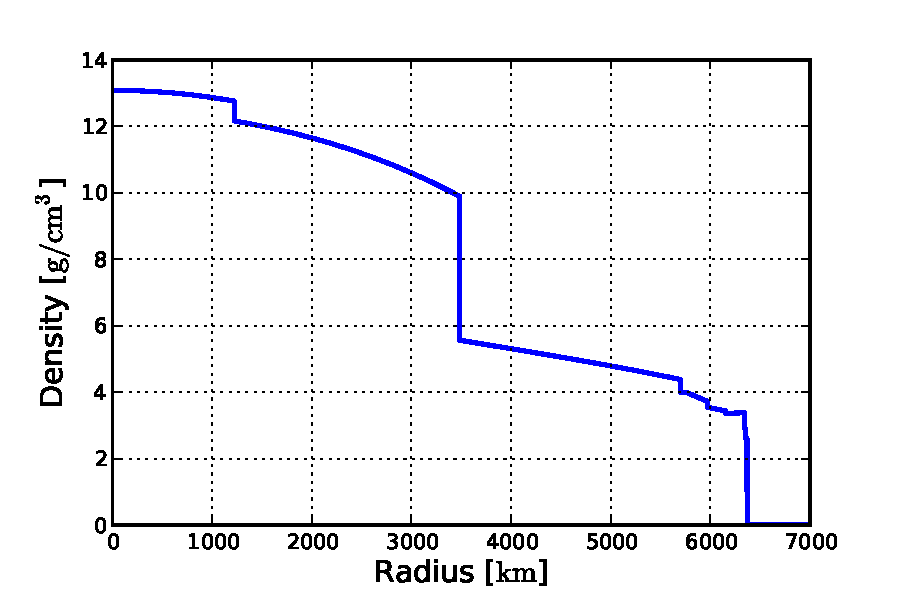
\includegraphics[width=0.7\textwidth]{PREM}
 \caption{The PREM Earth density profile \cite{PREM}.}
 \label{fig:PREM}
\end{figure}

In Figs.~\ref{fig:nue_to_numu} and \ref{fig:numu_to_numu}, the oscillation
probabilities for \nue to \numu and \numu to \numu are shown as examples. They
have been calculated using the AtmoWeights package that was developed by the
IceCube collaboration \cite{AtmoWeights} using the ``Preliminary Reference Earth
Model'' (PREM) \cite{PREM} for the Earth's density profile, shown in
Fig.~\ref{fig:PREM}. It is easily recognisable that the oscillation
probabilities for $\nu_\alpha \to \nu_\beta$ are in principle equal to those for
$\bar\nu_\alpha \to \bar\nu_\beta$, apart from the MSW resonance, easy to spot
in the energy range from 2 to \SI{10}{\GeV} for zenith angles below
$\coszen \approx -0.4$, that appears in neutrinos for the normal and in
antineutrinos for the inverted mass hierarchy (see Sec.~\ref{sec:matter_osc}).

\begin{figure}[p]
 \centering
 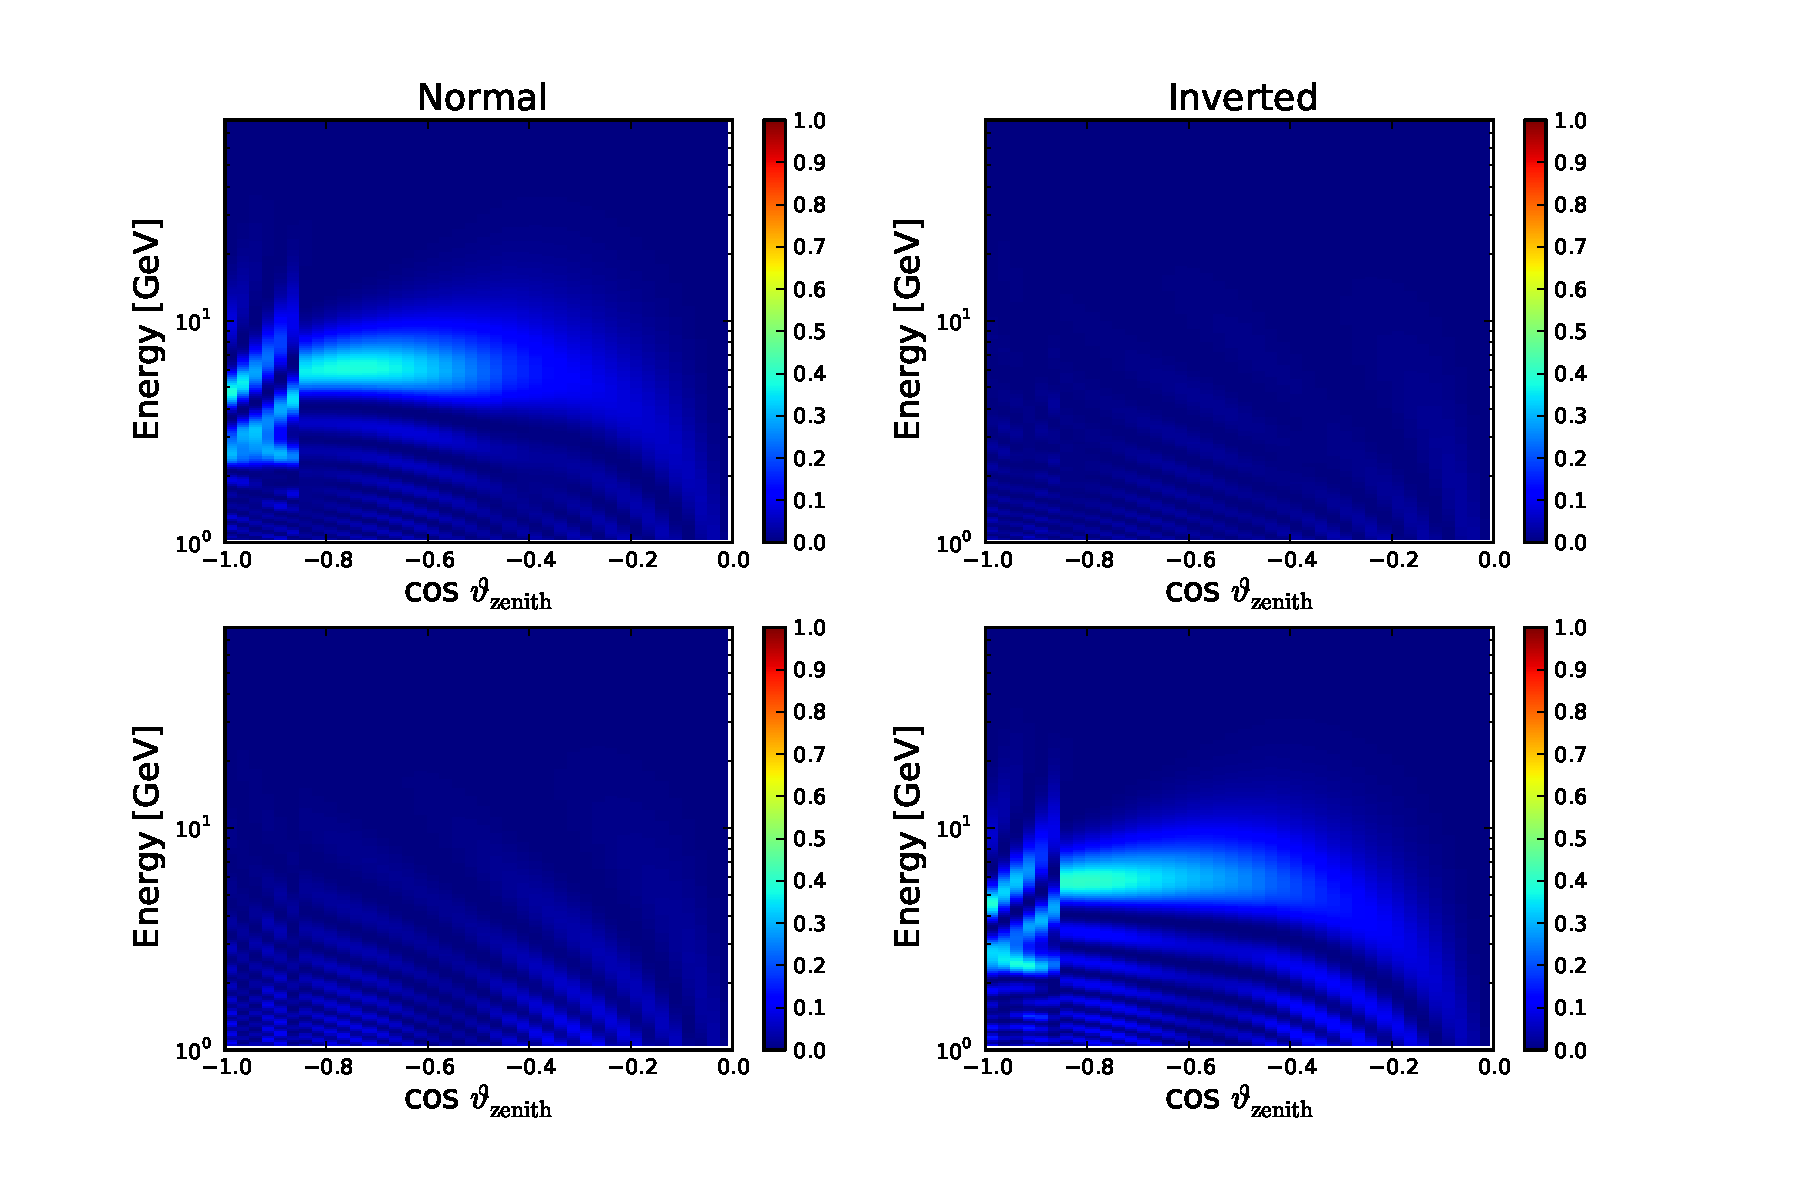
\includegraphics[width=0.95\textwidth]{osc_nue_to_numu}
 \caption{Oscillation probabilities for $\nue \to \numu$ (top) and $\nuebar \to
          \numubar$ (bottom) for normal and inverted hierarchy.}
 \label{fig:nue_to_numu}
\end{figure}
\begin{figure}[p]
 \centering
 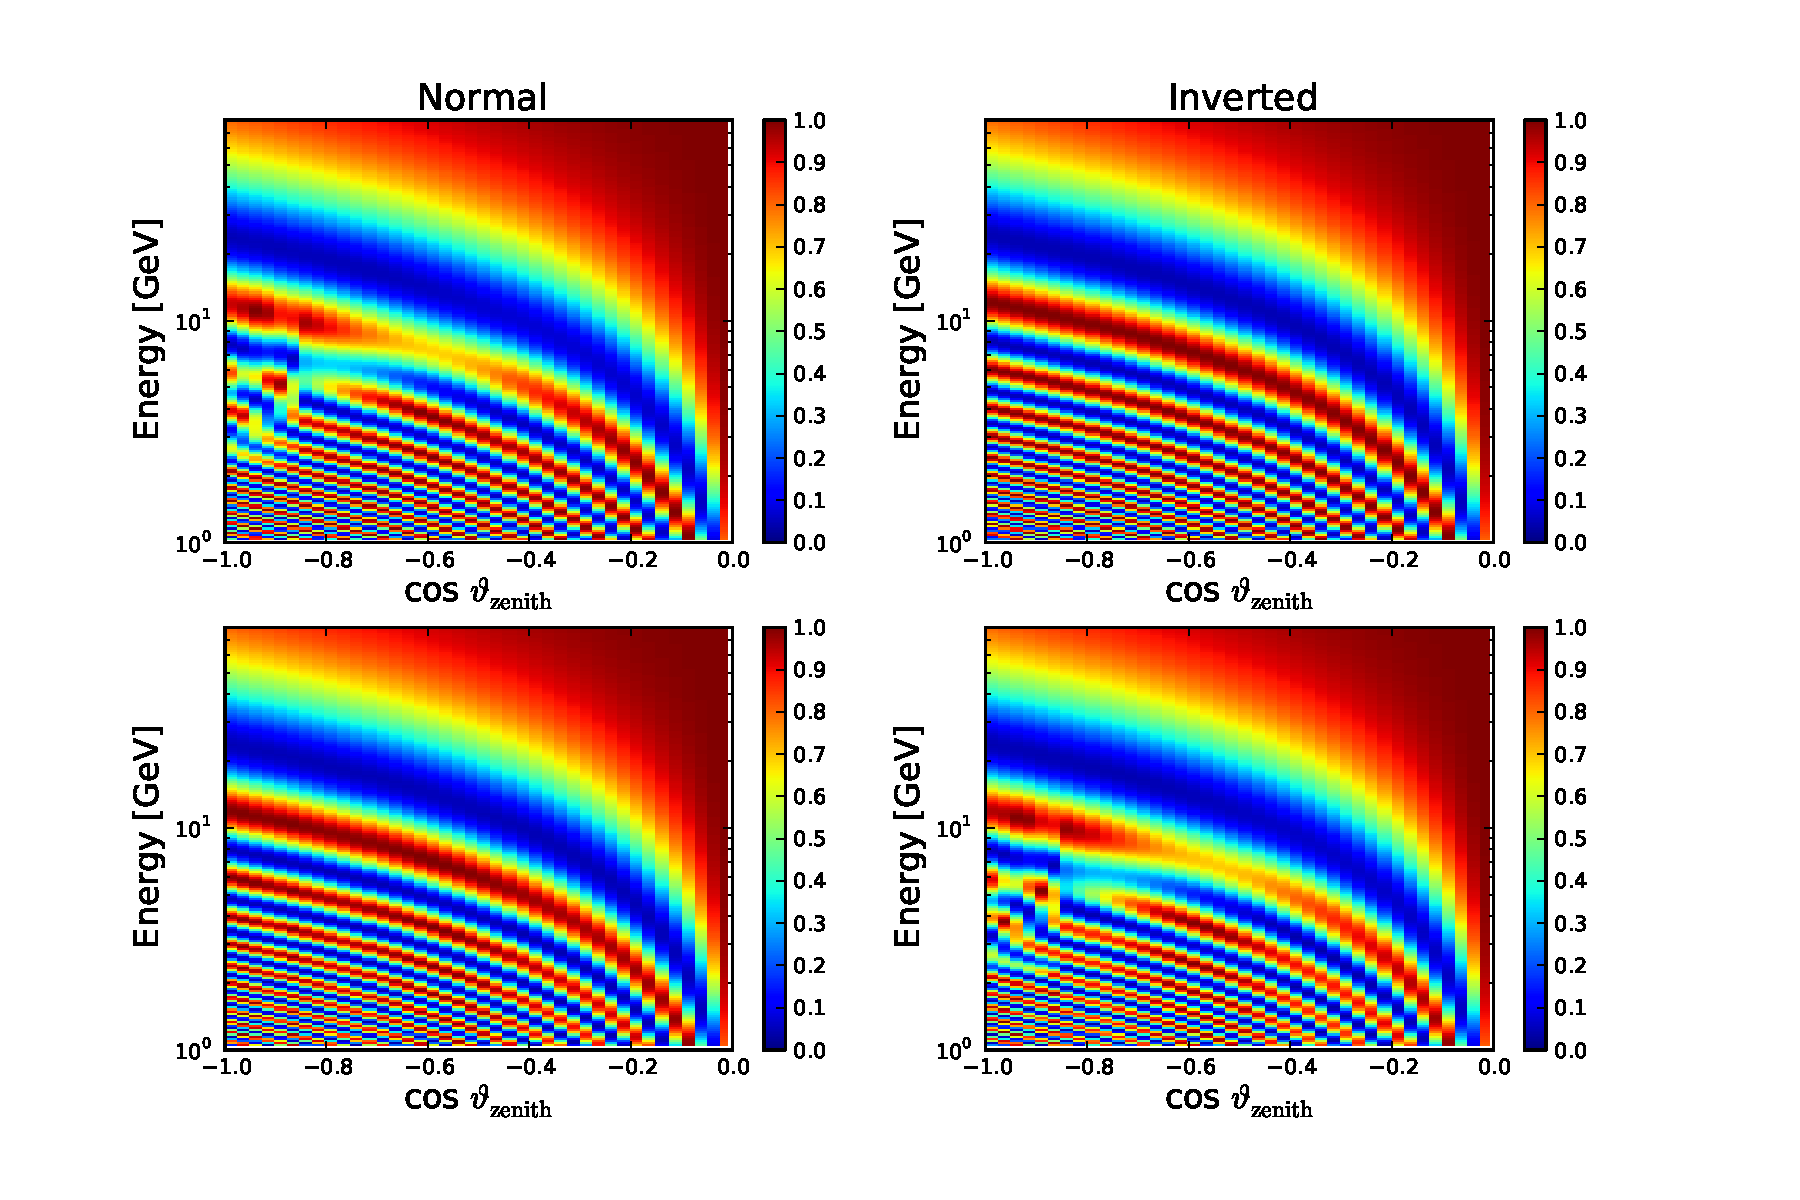
\includegraphics[width=0.95\textwidth]{osc_numu_to_numu}
 \caption{Oscillation probabilities for $\numu \to \numu$ (top) and $\numubar 
          \to \numubar$ (bottom) for normal and inverted hierarchy.}
 \label{fig:numu_to_numu}
\end{figure}

\enlargethispage{\baselineskip}
But since the fluxes of neutrinos and antineutrinos of the same flavour are 
essentially equal and PINGU cannot discriminate between them\footnote{The only
method to do this would be to identify the sign of the electrical charge of 
the lepton
produced in CC interactions. However it is unrealistic to generate the required
magnetic field in the antarctic glacier, where PINGU will be located (see
Secs.~\ref{sec:ICDC} and \ref{sec:PINGU}).}, the question is how the different
hierarchies can show up in the recorded data. Here the different cross-sections
for neutrinos and antineutrinos come into effect. As one can see from
Fig.~\ref{fig:NuXsec_GeV}, at the relevant energies just below \SI{10}{\GeV}
the cross section for antineutrino interactions with a hadronic target
material is about a factor of two lower than the one for neutrinos. Thus, the
MSW resonance will appear in the data in any case, but much more prominent if
the hierarchy is normal, as in this case roughly \sfrac{2}{3} of the
events---the neutrino-induced ones---are affected by it, while in the inverted
hierarchy case only the remaining third caused by antineutrinos is.

So the quantities of interest are the sum of neutrino and antineutrino events
for the different flavours at the energy and \coszen range where the MSW 
resonance is expected and how they differ assuming normal and inverted mass
hierarchy. To assess how significant the difference is in a given bin in the
($E$, \coszen) plane, we define a bin-wise \delchi similar to \cite{Akhmedov} 
as
\begin{equation}
 \delchi = \frac{N_\mathrm{NH} - N_\mathrm{IH}}{\sqrt{N_\mathrm{NH}}} \quad,
\end{equation}
where $N_\mathrm{NH}$ and $N_\mathrm{IH}$ are the expected number of events in
the normal and inverted hierarchy case, respectively. Plots of the event rates
and their weighted difference \delchi are shown in
Figs.~\ref{fig:true_akhmedov_nue} to \ref{fig:true_akhmedov_nutau}. In this
calculation not the bare cross-sections, but rather the \emph{effective
areas} for the different flavours enter, which also include the detection 
threshold
and selection efficiency of the detector. This will be discussed in detail in
Sec.~\ref{sec:sim_input}.

Comparing the different flavours, one notes that the largest overall scale of 
the
\delchi values appears in the \numu channel, but the contiguous regions of
either positive or negative \delchi are rather small and alternate rapidly.
Since a realistic detector has a limited resolution in reconstructing individual
events, it will be challenging to resolve these fine structures in the data. In
the \nue channel, the features are less pronounced, but more extended than for
\numu, offering a more robust measurement.

\begin{figure}[p]
 \centering
 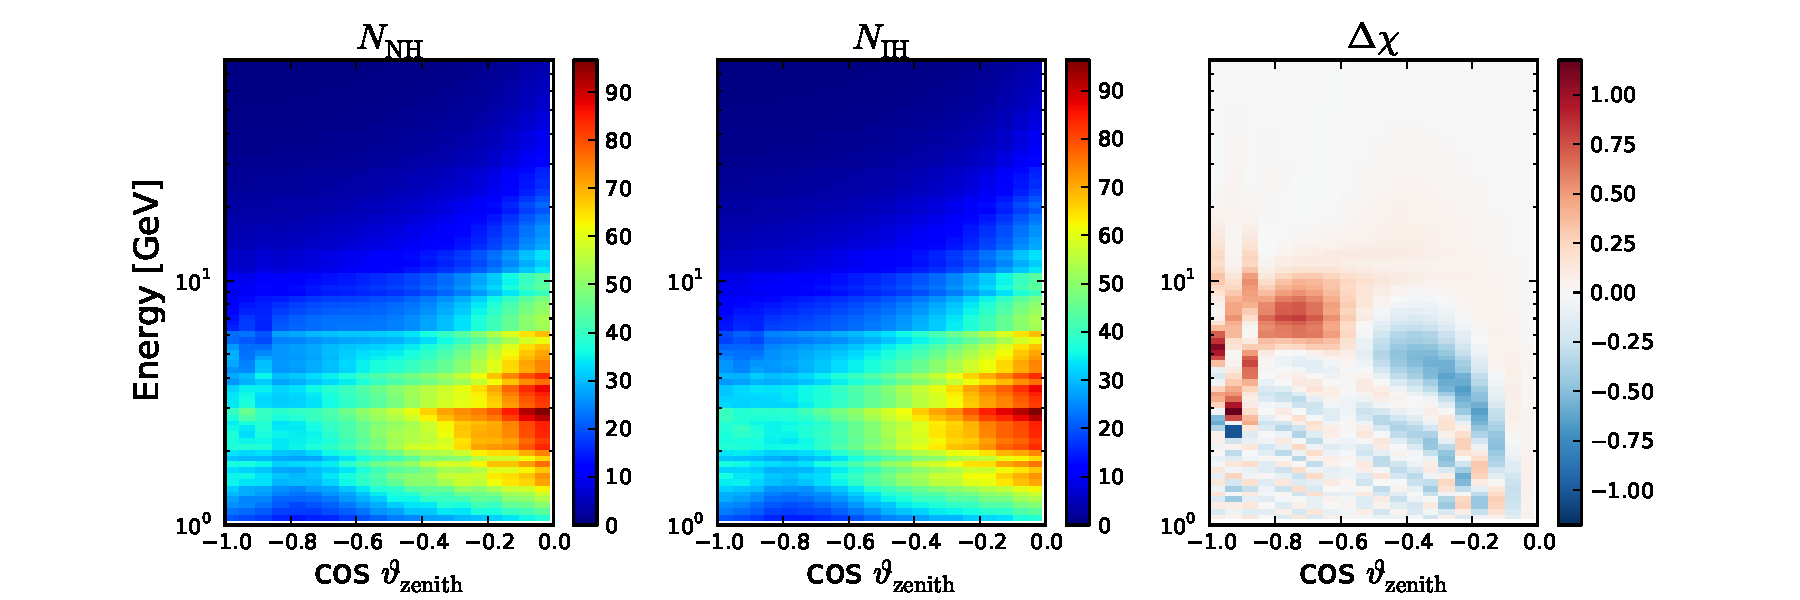
\includegraphics[width=\textwidth]{true_akhmedov_nue}
 \caption{Expected \nue + \nuebar CC event rates in PINGU (arbitrary units) for
    normal and inverted mass hierarchy and their weighted difference \delchi.}
 \label{fig:true_akhmedov_nue}
\end{figure}
\begin{figure}[p]
 \centering
 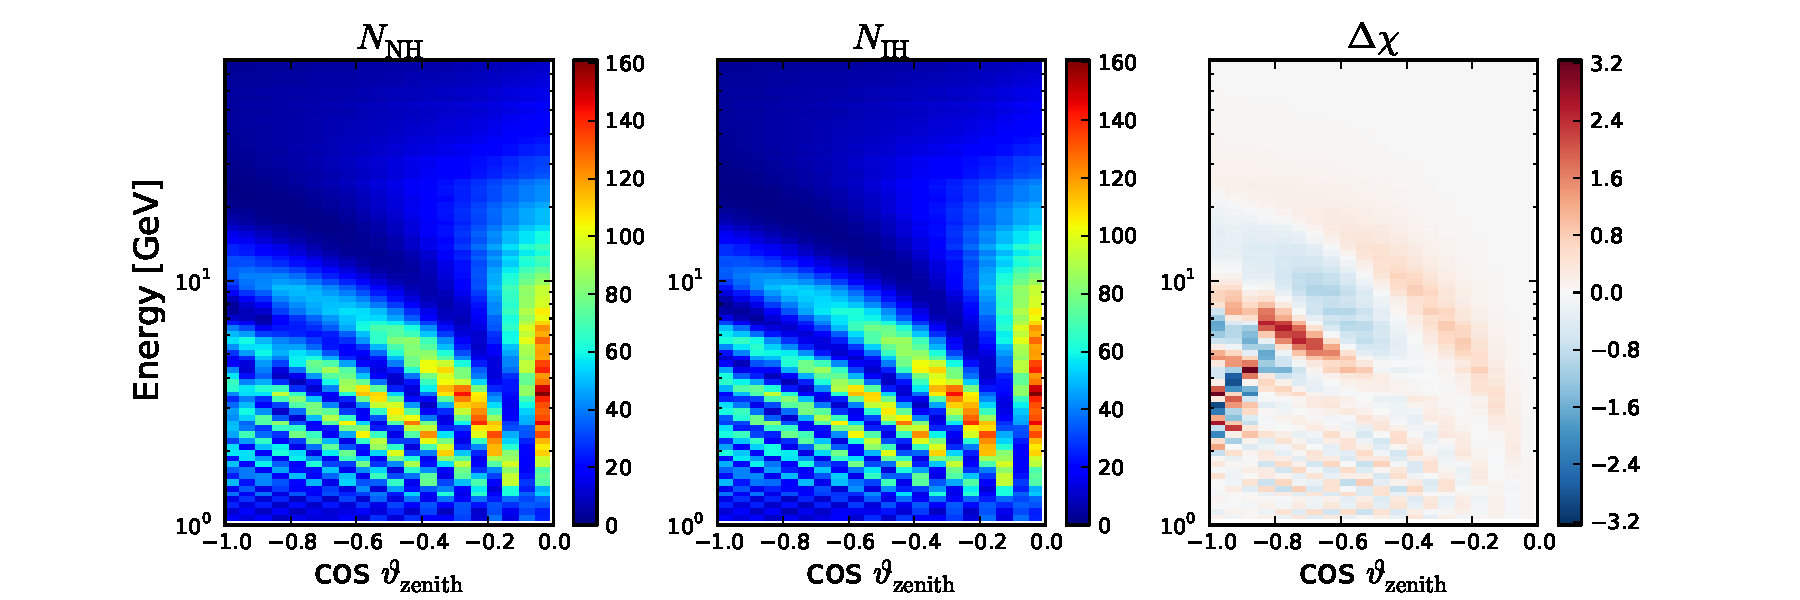
\includegraphics[width=\textwidth]{true_akhmedov_numu}
 \caption{Same as Fig.~\ref{fig:true_akhmedov_nue}, but for \numu + \numubar
    events}
 \label{fig:true_akhmedov_numu}
\end{figure}
\begin{figure}[p]
 \centering
 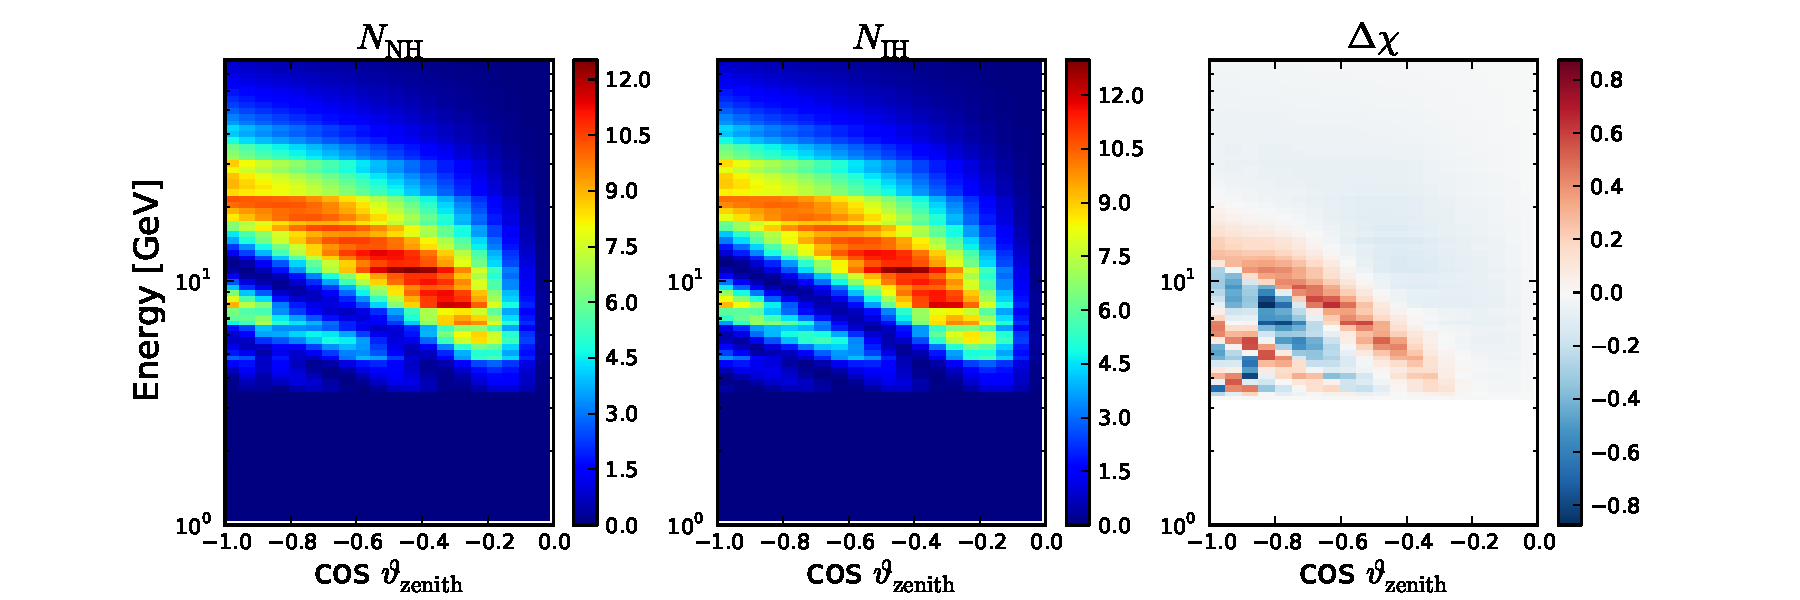
\includegraphics[width=\textwidth]{true_akhmedov_nutau}
 \caption{Same as Fig.~\ref{fig:true_akhmedov_nue}, but for \nutau + \nutaubar
    events}
 \label{fig:true_akhmedov_nutau}
\end{figure}
